\documentclass{homework}

\definecolor{bg}{rgb}{0.95,0.95,0.95}

\begin{document}
\frontpage{Þýðendur}{Scanner-NanoMorpho}{Guðmundur Óli Norland}{Egill Ragnarsson}{Snorri Agnarsson}

\begin{question}{Github}
  \href{https://github.com/slowpokesheep/thydendur/scanner}{Scanner}\\
\end{question}

\begin{question}{nanomorpho.jflex}
\end{question}
\begin{answer}
\begin{minted}[autogobble,tabsize=2, bgcolor=bg,breaklines,breakanywhere]{java}
  /*
  JFlex scanner for NanoMorpho

  Based on Snorri Agnarssons NanoLisp scanner.

  Authors:  Hjalti Geir Garðarsson
            Egill Ragnarsson
            Guðmundur Óli Norland
  
  Running the program:
    Compile:
      java -jar JFlex-full-1.7.0.jar nanomorpho.jflex
      javac NanoMorpho.java
    Run:
      java NanoMorpho <input_file> > <output_file>
  
  Use the makefile:
*/

import java.io.*;

%%

%public
%class NanoMorpho
%unicode
%byaccj

%{

// This part becomes a verbatim part of the program text inside
// the class, NanoMorpho.java, that is generated.

// Definitions of tokens:
static final int ERROR = -1;

static final int NAME = 1001;
static final int LITERAL = 1002;
static final int OPNAME = 1003;

// Decleration <decl>
static final int VAR = 1010;

// Expression <expr>
static final int RETURN = 1020;
static final int WHILE = 1021;

// If Expression <ifexpr>
static final int IF = 1030;
static final int ELSIF = 1031;
static final int ELSE = 1032;

// A variable that will contain lexemes as they are recognized:
private static String lexeme;

// This runs the scanner:
public static void main( String[] args ) throws Exception
{
  NanoMorpho lexer = new NanoMorpho(new FileReader(args[0]));
  int token = lexer.yylex();
  
  while(token != 0) {
    System.out.println(""+token+": \'"+lexeme+"\'");
    token = lexer.yylex();
  }
}

%}

/* Regular definitions */
_DIGIT=[0-9]
_FLOAT={_DIGIT}+\.{_DIGIT}+([eE][+-]?{_DIGIT}+)?
_INT={_DIGIT}+
_BOOL=(true|false)
_ESCAPE=\\b|\\t|\\n|\\f|\\r|\\\"|\\\'|\\\\|(\\[0-3][0-7][0-7])|(\\[0-7][0-7])|(\\[0-7])
_CHAR=\'([^\'\\]|{_ESCAPE})\'
_STRING=\"([^\"\\]|{_ESCAPE})*\"
_DELIM=[()\{\},;=]
_NAME=([:letter:]|{_DIGIT}|_)+
_OPNAME=([\+\-*/!%=><\:\^\~&|?])
_OPNAMETWO=(\=\=|\!\=|&&|\|\|)

%%

/* Scanning rules */

{_DELIM} {
  lexeme = yytext();
  return yycharat(0);
}

{_STRING} | {_FLOAT} | {_CHAR} | {_INT} | {_BOOL} | null {
  lexeme = yytext();
  return LITERAL;
}

"var" {
  lexeme = yytext();
  return VAR;
}

"return" {
  lexeme = yytext();
  return RETURN;
}

"while" {
  lexeme = yytext();
  return WHILE;
}

"if" {
  lexeme = yytext();
  return IF;
}

"elsif" {
  lexeme = yytext();
  return ELSIF;
}

"else" {
  lexeme = yytext();
  return ELSE;
}

{_NAME} {
  lexeme = yytext();
  return NAME;
}

{_OPNAME} | {_OPNAMETWO} {
  lexeme = yytext();
  return OPNAME;
}

// EOL character
";;;".*$ {
}

// White spaces are ignored
[ \t\r\n\f] {
}

// If all rules fail, return an error
. {
  lexeme = yytext();
  return ERROR;
}
\end{minted}
\end{answer}

\newpage

\begin{question}{makefile}
  
\end{question}
\begin{answer}
  \begin{minted}[autogobble,tabsize=2, bgcolor=bg,breaklines,breakanywhere]{makefile}
NanoMorpho.class: NanoMorpho.java
	javac NanoMorpho.java
NanoMorpho.java: nanomorpho.jflex
	java -jar jflex-full-1.7.0.jar nanomorpho.jflex

clean:
	rm -rf *~ NanoMorpho.class NanoMorpho.java

test: test1 test2 test3

test1:
	java NanoMorpho tests/test1.s | ../util/test_output.py

test2:
	java NanoMorpho tests/test2.s | ../util/test_output.py

test3:
	java NanoMorpho tests/test3.s | ../util/test_output.py
  \end{minted}
\end{answer}

\newpage

\begin{question}{Test output}
  \textbf{\underline{Test 1}}
  \begin{verbatim}
    main(i, j) {
      var r, s;
      var t = "Hallo";

      writeln("Hello World!");
    }
  \end{verbatim}
  \textbf{\underline{Test 1}}
  \begin{verbatim}
    my_function(j, k) {

      if (j > k) {
        return j;
      }
      elsif (k > j) {
        return k;
      }
      else {
        return 0;
      }
    }
  \end{verbatim}
  \textbf{\underline{Test 1}}
  \begin{verbatim}
    var bubbi_byggir = false;
    if (!bubbi_byggir && bubbi_byggir == false) {
    	writeln("Bubbi er ekki að byggja núna! Úps!");
    };
    var x = 5;
    while (x==2 && x<-123 || (x==321 && x!=5)) {
    	writeln("þetta gerist aldrei LOL! \b \t \n \r");
    };
    $@
  \end{verbatim}
\end{question}
\begin{answer}
  \begin{figure}[H]
    \centering
    \caption*{Test\_1}
    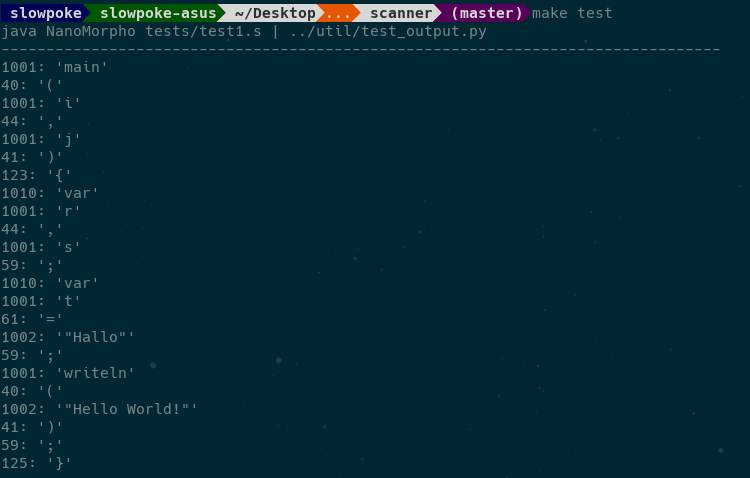
\includegraphics[width=0.8\textwidth]{test1.png}
  \end{figure}
  \begin{figure}[H]
    \centering
    \caption*{Test\_3}
    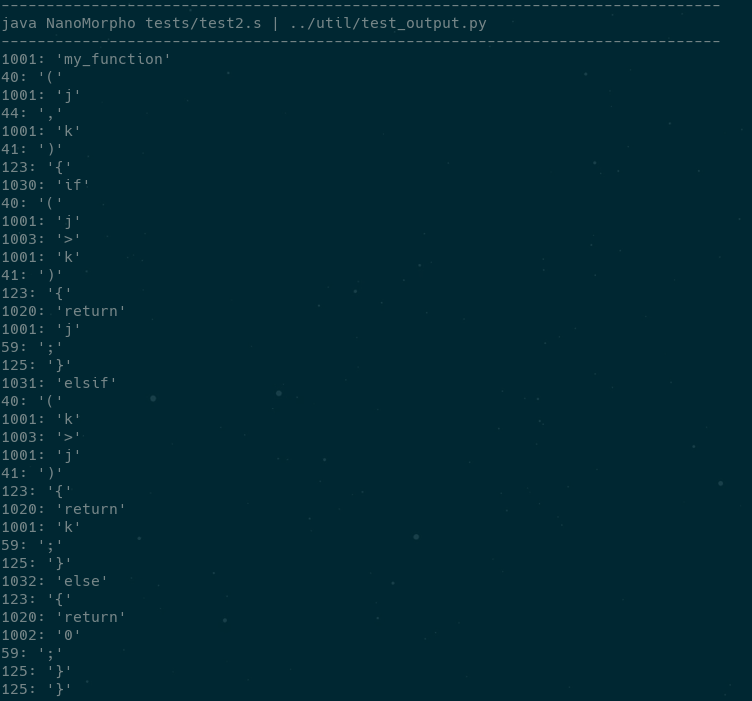
\includegraphics[width=0.8\textwidth]{test2.png}
  \end{figure}
  \begin{figure}[H]
    \centering
    \caption*{Test\_3}
    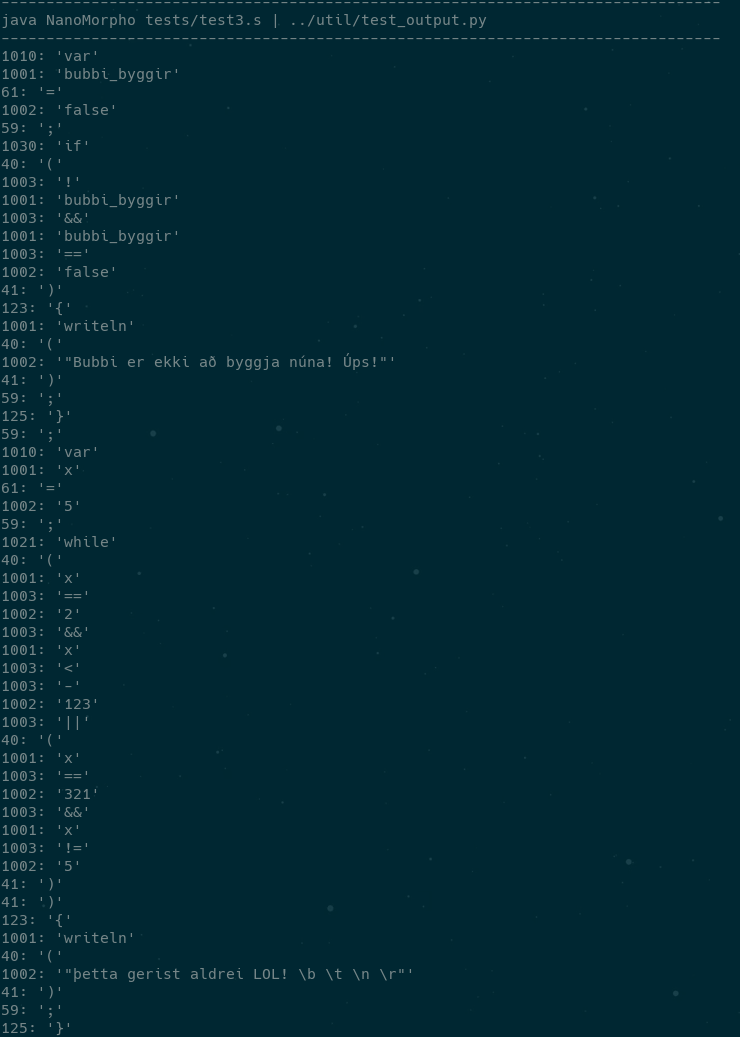
\includegraphics[width=0.8\textwidth]{test3_a.png}
  \end{figure}
  \begin{figure}[H]
    \centering
    \caption*{Test\_3}
    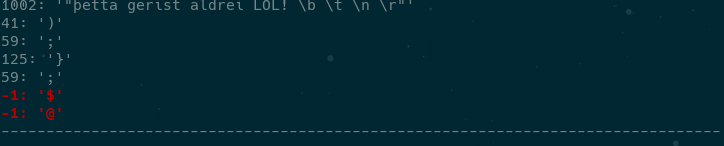
\includegraphics[width=0.8\textwidth]{test3_b.png}
  \end{figure}
\end{answer}

\end{document}
